\section{Mathematical model}
\label{section:lung_model}
%We will now introduce the quasi-static fully incompressible poroelasticity equations, used for modelling the lung parenchyma, a simple fluid network model to model the airway tree, and outline how these two parts are coupled together.

\subsection{A poroelastic model for lung parenchyma} 
Having made the assumptions in section \ref{sec:assumptions} for the tissue we are left with the large deformation quasi-static incompressible poroelastic model (\ref{eqn:simple_mixture_model}).%
\subsubsection{Constitutive laws.}
\label{sec:constitutive}
To close the poroelastic model for the tissue (\ref{eqn:simple_mixture_model}) we need to choose constitutive laws for the permeability and strain energy. We will use the same permeability law that has already been proposed in \cite{kowalczyk1994modelling} to model lung parenchyma,
\begin{equation}
\bb{k}_{0} = {k}_{0} \left( J \frac{  \phi  }{\phi_{0}} \right)^{2/3} \boldsymbol{I}.
\label{eqn:perm_law}
\end{equation}
%
Exponential strain energy laws for lung parenchyma exist, for example the popular law by \cite{fung1975stress}. However little is known about how the constants in these laws should be interpreted and altered to model weakening of the tissue in an diseased state. Further, the constants in these laws are thought to have no physical meaning \cite{tawhai2009supine}. To make the interpretation of the elasticity constants and dynamics of the model as simple as possible we chose a Neo-Hookean law taken from \cite{wriggers2008nonlinear}, with the penalty term chosen such that $0\leq\phi<1$,
%
%from \cite[eqn. (3.119)]{wriggers2008nonlinear},
\begin{equation}
W(\bb{C})=\frac{\mu}{2}(\mbox{tr}(\boldsymbol{C})-3)+\frac{\lambda}{4}(J^{2}-1)-(\mu+\frac{\lambda}{2})\mbox{ln}(J-1+\phi_{0}).
\label{eqn:Neo_Hookean}
\end{equation}
The material parameters $\mu$ and $\lambda$ can be related to the more familiar Young's modulus $E$ and the Poisson ratio $\nu$ by $\mu=\frac{E}{2(1+\nu)}$ and  $\lambda=\frac{E\nu}{(1+\nu)(1-2\nu)}$. The values of these constants for modelling lung tissue have been investigated \cite{zhang2004technical,werner2009patient,de1981model} and are shown in Table \ref{tab:lung_sim_parameters}.


\subsection{A network flow model for the airway tree}
The flow rate $Q_{i}$ through the $ith$ pipe segment in the fluid network is given by the pressure-flow relationship
\begin{equation}
 \label{pois_flow_eqn}
 P_{i,1} - P_{i,2} = R_{i} Q_{i},
\end{equation}
where $R_{i}=\frac{8l\mu_{f}}{\pi r^{4}}$ is the Poiseuille flow resistance of a pipe segment ($r$ is the radius, $l$ is the length of the pipe, $\mu_{f}$ is the dynamic viscosity) and $P_{i, 1}$ and $P_{i,2}$ are the pressures at the proximal and distal nodes of the pipe segment, respectively. We also have conservation of flow at branches such that
\begin{equation}
 Q_{i}  = \sum_{Q_{i,j} \in Q_{i}} Q_{i,j},
\end{equation}
where $Q_{i,j}$ are the flow rates of the children branches of the $i$th flow segment. The outlet pressure of the fluid network is set using the boundary condition $P_{0}=\hat{P}$.



\subsubsection{Coupling the fluid network to the poroelastic model.}
We introduce subdomains to identify the region of the domain that is supplied with fluid from a specific branch of the fluid network and returns fluid through that branch. We construct an approximate Voronoi tesselation based on the terminal end locations of the fluid network, so that the $i$th subdomain $\Omega_{t}^{i}$ is the set of finite elements whose centroids are closer to the  $i$th inlet than any of the other inlets. Obviously we have $\Omega_{t}=\sum_{i}^{N} \Omega_{t}^{i}$. The introduction of subdomains allows each endpoint of the fluid network to supply and remove fluid from the poroelastic medium at different spatial locations.   
%
%%% CONTINOUS ONLY %%%%%%%%%%%%%
%
The $i$th subdomain $\Omega_{t}^{i}$ is defined as the volume closest to the position of the $i$th inlet, denoted by $\mbox{pos}(P_{di})$. 
\begin{equation}
\Omega_{t}^{i} := \left\lbrace \boldsymbol{x} \in \Omega_{t} : ||\boldsymbol{x} -\mbox{pos}(P_{di}) || <  ||\boldsymbol{x} -\mbox{pos}(P_{dj}) ||, \;j=1,2...,N \;, j \neq i \right\rbrace.
 \label{subdomain_definition}
\end{equation}
For notational purposes we have added subscript $di$ to the most distal branches that have no further conducting branches coming from them but instead enter a group of acinar units (approximated by the poroelastic model). In Figure \ref{fig:domains_cont} we demonstrate how the domain is coupled to the distal branches using a simple 2D example. The discretization of this 2D example is described in section \ref{sec:coupling_appendix}.


%If we descrtize the space using triangles and employ a piecewise constant pressure approximation (one node at the center of each element), then the resutling coupling . The elements are coupled to the distal branch end poiunts as is shown in Figure \ref{fig:coupling_disc1}. Once we refine the mesh the discretized tend to the domain subdivision of the original problem, as is shown in \ref{fig:coupling_disc2}. This highlights that the numerical approximation is not mesh dependent, provided a fine enough mesh discretisation is used.
%
%

\begin{figure}[h]
\centering
{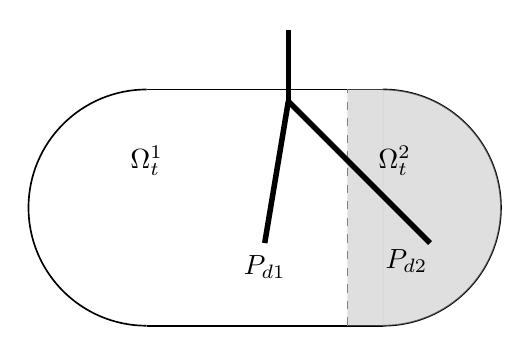
\begin{tikzpicture}[scale=1.5]
	%Domain	
	\draw[semithick] (1,2) arc (90:270:1cm);
	\draw[semithick] (3,0) arc (-90:90:1cm);
	\draw[semithick] (1,2) -- (3,2);
	\draw[semithick] (1,0) -- (3,0);
	%Shade Omega_2
	\draw[draw=none,fill=black!25,fill opacity=0.5] (3,0) arc (-90:90:1cm) -- (3,2) -- (3,0)  -- (3,2);
\draw[draw=none, fill=black!25,fill opacity=0.5] (2.7,0) -- (2.7,2)  -- (3.005,2)    -- (3.005,0)  -- (2.7,0);
    %Division
    \draw[dashed,color=gray] (2.7,0) -- (2.7,2);	
	%TREE
    \draw[line width=2pt] (2.2,1.9) -- (2.2,2.5);
    \draw[line width=2pt] (3.4,0.7) -- (2.2,1.9);
    \draw[line width=2pt] (2,0.7) -- (2.2,1.9);
    
	%Labelling
	\draw (3.2,0.55) node {$P_{d2}$};
	\draw (3.1,1.4) node {  $\Omega_{t}^{2}$};
	\draw (2,0.5) node {$P_{d1}$};
	\draw (1,1.4) node {  $\Omega_{t}^{1}$};	
\end{tikzpicture}
} 
\caption{A simple example of a 2D domain being split into two subdomains dependent on the position of end points of the fluid network.} 
\label{fig:domains_cont}
\end{figure}
%
%
%
%
%%%% DISCRETIZED ONLY %%%%%%%%%%%%%
%
%The $i$th subdomain $\Omega_{t}^{i}$ is the set of finite elements whose centroids are closer to the  $i$th inlet than any of the other inlets.
%, denoted by $\mbox{pos}(P_{di})$.
%\begin{equation}
%\Omega_{t}^{i} := \left\lbrace \boldsymbol{x} \in \Omega_{t} : ||\boldsymbol{x} -\mbox{pos}(P_{di}) || <  ||\boldsymbol{x} -\mbox{pos}(P_{dj}) ||, \;j=1,2...,N \;, j \neq i \right\rbrace.
% \label{subdomain_definition}
%\end{equation}
%For notational purposes we have added subscript $di$ to the most distal branches that have no further conducting branches coming from them but instead enter a group of acinar units (approximated by the poroelastic model). In Figure \ref{fig:domains_cont} we demonstrate how the domain is coupled to the distal branches using a simple 2D example.

%If we descrtize the space using triangles and employ a piecewise constant pressure approximation (one node at the center of each element), then the resutling coupling . The elements are coupled to the distal branch end poiunts as is shown in Figure \ref{fig:coupling_disc1}. Once we refine the mesh the discretized tend to the domain subdivision of the original problem, as is shown in \ref{fig:coupling_disc2}. This highlights that the numerical approximation is not mesh dependent, provided a fine enough mesh discretisation is used.
%
%
%\begin{figure}[h]
%\centering
%  \subfloat[]{\begin{tikzpicture}[scale=1.15]
%	%Domain	
%	\draw[semithick] (1,2) arc (90:270:1cm);
%	\draw[semithick] (3,0) arc (-90:90:1cm);
%	\draw[semithick] (1,2) -- (3,2);
%	\draw[semithick] (1,0) -- (3,0);
%	%Shade Omega_2
%	\draw[line width=0pt,draw opacity=0,fill=black!25,fill opacity=0.5] (3,0) arc (-90:90:1cm) -- (3,2)
%      -- (3,0)  -- (3,2);
%	\draw[line width=0pt,draw opacity=0,fill=black!25,fill opacity=0.5] (2.7,0) -- (2.7,2)  -- (3,2)    -- (3,0)  -- (2.7,0);
%    %Division
%    \draw[dashed,color=gray] (2.7,0) -- (2.7,2);	
%	%TREE
%    \draw[line width=2pt] (2.2,1.9) -- (2.2,2.5);
%    \draw[line width=2pt] (3.4,0.7) -- (2.2,1.9);
%    \draw[line width=2pt] (2,0.7) -- (2.2,1.9);
%
%	%Labelling
%	\draw (3.2,0.55) node {$P_{d2}$};
%	\draw (3.1,1.4) node {  $\Omega_{t}^{2}$};
%	\draw (2,0.5) node {$P_{d1}$};
%	\draw (1,1.4) node {  $\Omega_{t}^{1}$};	
%\end{tikzpicture}
%\label{fig:domains_cont}
%}
%\subfloat[]{\begin{tikzpicture}[scale=1.15]
%  %Coarse discretisation
%  \draw[semithick,fill=black!2,fill opacity=0.5]
%    (0,1) to (1,2) to  (2,1) to (0,1) ;
%  \draw[semithick,fill=black!2,fill opacity=0.5]
%    (0,1) to (1,0) to  (2,1) to (0,1) ;
%  \draw[semithick,fill=black!2,fill opacity=0.5]
%    (1,2) to (2,1) to  (3,2) to (1,2) ;
%   \draw[semithick,fill=black!2,fill opacity=0.5]
%    (1,0) to (2,1) to  (3,0) to (1,0) ;
%    \draw[semithick,fill=black!25,fill opacity=0.5]
%    (2,1) to (3,2) to  (4,1) to (2,1) ;
%  \draw[semithick,fill=black!25,fill opacity=0.5]
%    (2,1) to (3,0) to  (4,1) to (2,1) ;
%
%   %TREE
%  \draw[line width=2pt] (2.2,1.9) -- (2.2,2.5);
%  \draw[line width=2pt] (3.4,0.7) -- (2.2,1.9);
%  \draw[line width=2pt] (2,0.7) -- (2.2,1.9);
%    		     	
%	%Labelling
%	%\draw (3.2,0.55) node {$P_{d2}$};
%	\draw (3.1,1.4) node {  $\Omega_{t}^{2}$};
%	%\draw (2,0.5) node {$P_{d1}$};
%	\draw (1,1.4) node {  $\Omega_{t}^{1}$};	
%\end{tikzpicture}
%\label{fig:coupling_disc1}
%}
%\subfloat[]{\begin{tikzpicture}[scale=1.15]
%
%  %Top left tri
%  \draw[semithick,fill=black!2,fill opacity=0.5]
%    (0,1) to (0.3,1.7141) to  (1,1) to (0,1) ;
%   \draw[semithick,fill=black!2,fill opacity=0.5]
%    (1,1) to (1.5,1.5) to  (2,1) to (1,1) ;
%  \draw[semithick,fill=black!2,fill opacity=0.5]
%    (0.3,1.7141) to (1,2) to  (1.5,1.5) to (0.3,1.7141) ;
%    \draw[semithick,fill=black!2,fill opacity=0.5]
%    (0.3,1.7141) to (1.5,1.5) to  (1,1) to (0.3,1.7141) ;
%
%   %Top right tri
%   \draw[semithick,fill=black!25,fill opacity=0.5]
%    (2.5,1.5) to (3,2) to  (3.7,1.7141) to (2.5,1.5) ;
%       \draw[semithick,fill=black!25,fill opacity=0.5]
%    (2.5,1.5) to (3.7,1.7141) to  (3,1) to (2.5,1.5) ;
%  \draw[semithick,fill=black!2,fill opacity=0.5]
%    (2,1) to (2.5,1.5) to  (3,1) to (2,1) ;
%   \draw[semithick,fill=black!25,fill opacity=0.5]
%   (3,1) to (3.7,1.7141) to  (4,1) to (3,1) ;
%
%   %Bottom left
%   \draw[semithick,fill=black!2,fill opacity=0.5]
%    (0,1) to (0.3,0.2859) to  (1,1) to (0,1) ;
%   \draw[semithick,fill=black!2,fill opacity=0.5]
%    (1,1) to (1.5,0.5) to  (2,1) to (1,1) ;
%  \draw[semithick,fill=black!2,fill opacity=0.5]
%    (0.3,0.2859) to (1,0) to  (1.5,0.5) to (0.3,0.2859) ;
%    \draw[semithick,fill=black!2,fill opacity=0.5]
%    (0.3,0.2859) to (1.5,0.5) to  (1,1) to (0.3,0.2859) ;
%
%
%    %Bottom right
%  \draw[semithick,fill=black!25,fill opacity=0.5]
%    (2.5,0.5) to (3,0) to  (3.7,0.2859) to (2.5,0.5) ;
%       \draw[semithick,fill=black!25,fill opacity=0.5]
%    (2.5,0.5) to (3.7,0.2859) to  (3,1) to (2.5,0.5) ;
%  \draw[semithick,fill=black!2,fill opacity=0.5]
%    (2,1) to (2.5,0.5) to  (3,1) to (2,1) ;
%   \draw[semithick,fill=black!25,fill opacity=0.5]
%   (3,1) to (3.7,0.2859) to  (4,1) to (3,1) ;
%
%  %Bottom middle - to do
%  \draw[semithick,fill=black!2,fill opacity=0.5]
%    (1.5,0.5) to (2,1) to  (2.5,0.5) to (1.5,0.5) ;
%  \draw[semithick,fill=black!2,fill opacity=0.5]
%    (1,0) to (1.5,0.5) to  (2,0) to (1,0) ;
%  \draw[semithick,fill=black!2,fill opacity=0.5]
%    (2,0) to (2.5,0.5) to  (3,0) to (2,0) ;
%  \draw[semithick,fill=black!2,fill opacity=0.5]
%    (1.5,0.5) to (2,0) to  (2.5,0.5) to (1.5,0.5) ;
%
%  %Top Middle
%  \draw[semithick,fill=black!2,fill opacity=0.5]
%    (1.5,1.5) to (2,1) to  (2.5,1.5) to (1.5,1.5) ;
%  \draw[semithick,fill=black!2,fill opacity=0.5]
%    (1,2) to (1.5,1.5) to  (2,2) to (1,2) ;
%  \draw[semithick,fill=black!2,fill opacity=0.5]
%    (2,2) to (2.5,1.5) to  (3,2) to (2,2) ;
%  \draw[semithick,fill=black!2,fill opacity=0.5]
%    (1.5,1.5) to (2,2) to  (2.5,1.5) to (1.5,1.5) ;
%   %TREE
%   \draw[line width=2pt] (2.2,1.9) -- (2.2,2.5);
%   \draw[line width=2pt] (3.4,0.7) -- (2.2,1.9);
%   \draw[line width=2pt] (2,0.7) -- (2.2,1.9);	
%	%Labelling
%	%\draw (3.2,0.55) node {$P_{d2}$};
%	\draw (3.1,1.4) node {  $\Omega_{t}^{2}$};
%	%\draw (2,0.5) node {$P_{d1}$};
%	\draw (1,1.4) node {  $\Omega_{t}^{1}$};	
%\end{tikzpicture}
%\label{fig:coupling_disc2}
%}
%\caption{(a) A simple example of a 2D domain being split into two subdomains dependent on the position of end points of the fluid network. (b) Coupling between the discretized domain and the fluid network using a piecewise constant pressure approximation. (c) Coupling between the discretized domain and the fluid network after mesh refinement.}
%\label{fig:coupling}
%\end{figure}
%
 We couple the airway network to the poroelastic domain by adding the flow contribution from each distal airway to the poroelastic domain as a source term in the poroelastic mass conservation equation (\ref{eqn:mixture_mass_reform}), such that
\begin{equation}
 \nabla \cdot ( \boldsymbol{v}^{s} + \boldsymbol{z}) = Q_{di} \;\;\;\; \mbox{in}\;\Omega_{t}^{i}.
 \label{fluid_mass_coupling}
\end{equation}
We also couple the airway network to the poroelastic domain by setting the average pressure in the poroelastic domain within $\Omega_{t}^{i}$ to be the same as the corresponding distal pressure node $P_{di}$ of the flow segment $Q_{di}$,
  \begin{equation}
  \frac{1}{|\Omega_{t}^{i}|} \int_{\Omega_{t}^{i}} p = P_{di},
   \label{pressure_coupling}
 \end{equation}
where $|\Omega_{t}^{i}|$ denotes the volume of the segment $\Omega_{t}^{i}$. Equation (\ref{pressure_coupling}) enforces the assumption that the end pressure in a terminal bronchiole is the same as the alveolar pressure in the surrounding tissue. %If we discretize the space using triangles and employ a piecewise constant pressure approximation (one node at the center of each element), the resulting coupling for a simple 2D example is shown in Figure \ref{fig:coupling_disc1}. Once we refine the mesh (Figure \ref{fig:coupling_disc2}), the discretized division of subdomains tends to the subdivision of the original problem (Figure \ref{fig:domains_cont}).
%This highlights that the numerical approximation is not mesh dependent, provided a fine enough mesh discretisation is used.
%
%
\subsection{Summary of the coupled lung model.}
\label{section:model_eqn_summary}
To solve the coupled poroelastic-fluid-network lung model we need to find $\boldsymbol{\chi}(\boldsymbol{X},t)$,  $\boldsymbol{z}(\boldsymbol{x},t)$, $p(\boldsymbol{x},t)$, $P_{i}$ and $Q_{i}$ such that
\begin{subequations}
\begin{align}
\label{eqn:mixture_momentum_reform_full}
-\nabla \cdot( \boldsymbol{\sigma}_{e} -p\boldsymbol{I}) = \rho\boldsymbol{f} \;\;\; \mbox{in} \; \Omega_{t},\\
\label{eqn:fluid_momentum_reform_full}
{\perm^{-1}\boldsymbol{z}} + \nabla p =  \rho^{f}\boldsymbol{f} \;\;\; \mbox{in} \; \Omega_{t}, \\
\label{eqn:mixture_mass_reform_full}
 \nabla \cdot ( \boldsymbol{v}^{s} + \boldsymbol{z}) = Q_{di} \;\;\;\; \mbox{in}\;\Omega_{t}^{i},\\
\boldsymbol{\chi} =\boldsymbol{X}+\boldsymbol{u}_{D}   \;\;\; \mbox{on}\; \Gamma_{d},
\\
(\boldsymbol{\sigma}_{e}-p\boldsymbol{I})\boldsymbol{n} = \boldsymbol{t}_{N}   \;\;\; \mbox{on}\; \Gamma_{t},
\\
\boldsymbol{z} \cdot \boldsymbol{n} = {q_{D}}   \;\;\; \mbox{on}\; \Gamma_{f},
\\
p = p_{D}   \;\;\; \mbox{on}\; \Gamma_{p},
\\
\boldsymbol{\chi}(0) = \boldsymbol{X} + \boldsymbol{u}^{0},   \;\;\;  \mbox{in}\;\Omega_{0},\\ %\hline
\label{eqn:tree_pressure_bc}
P_{0}=\hat{P},\\
\label{eqn:tree_flow}
  P_{i,1} - P_{i,2} = R_{i} Q_{i},\\
  \label{eqn:tree_mass}
Q_{i}  = \sum_{Q_{i,j} \in Q_{i}} Q_{i,j},\\
  \label{eqn:pressure_coupling}
\frac{1}{|\Omega_{t}^{i}|} \int_{\Omega_{t}^{i}} p = P_{di}.
\end{align}
\label{eqn:full_model}
\end{subequations}
%
